% RISC-V Single-Cycle Datapath  —  derived from Core_Datapath.v
% Blocks: PC, Instr Memory, Register File, Extend, SrcA/SrcB muxes,
%         ALU, Data Memory, CSR File, Result Mux, PC+4 / PC+Imm adders, PC Mux
\documentclass[border=10pt]{standalone}
\usepackage{tikz}
\usetikzlibrary{positioning, arrows.meta, calc, shapes.geometric}

\begin{document}
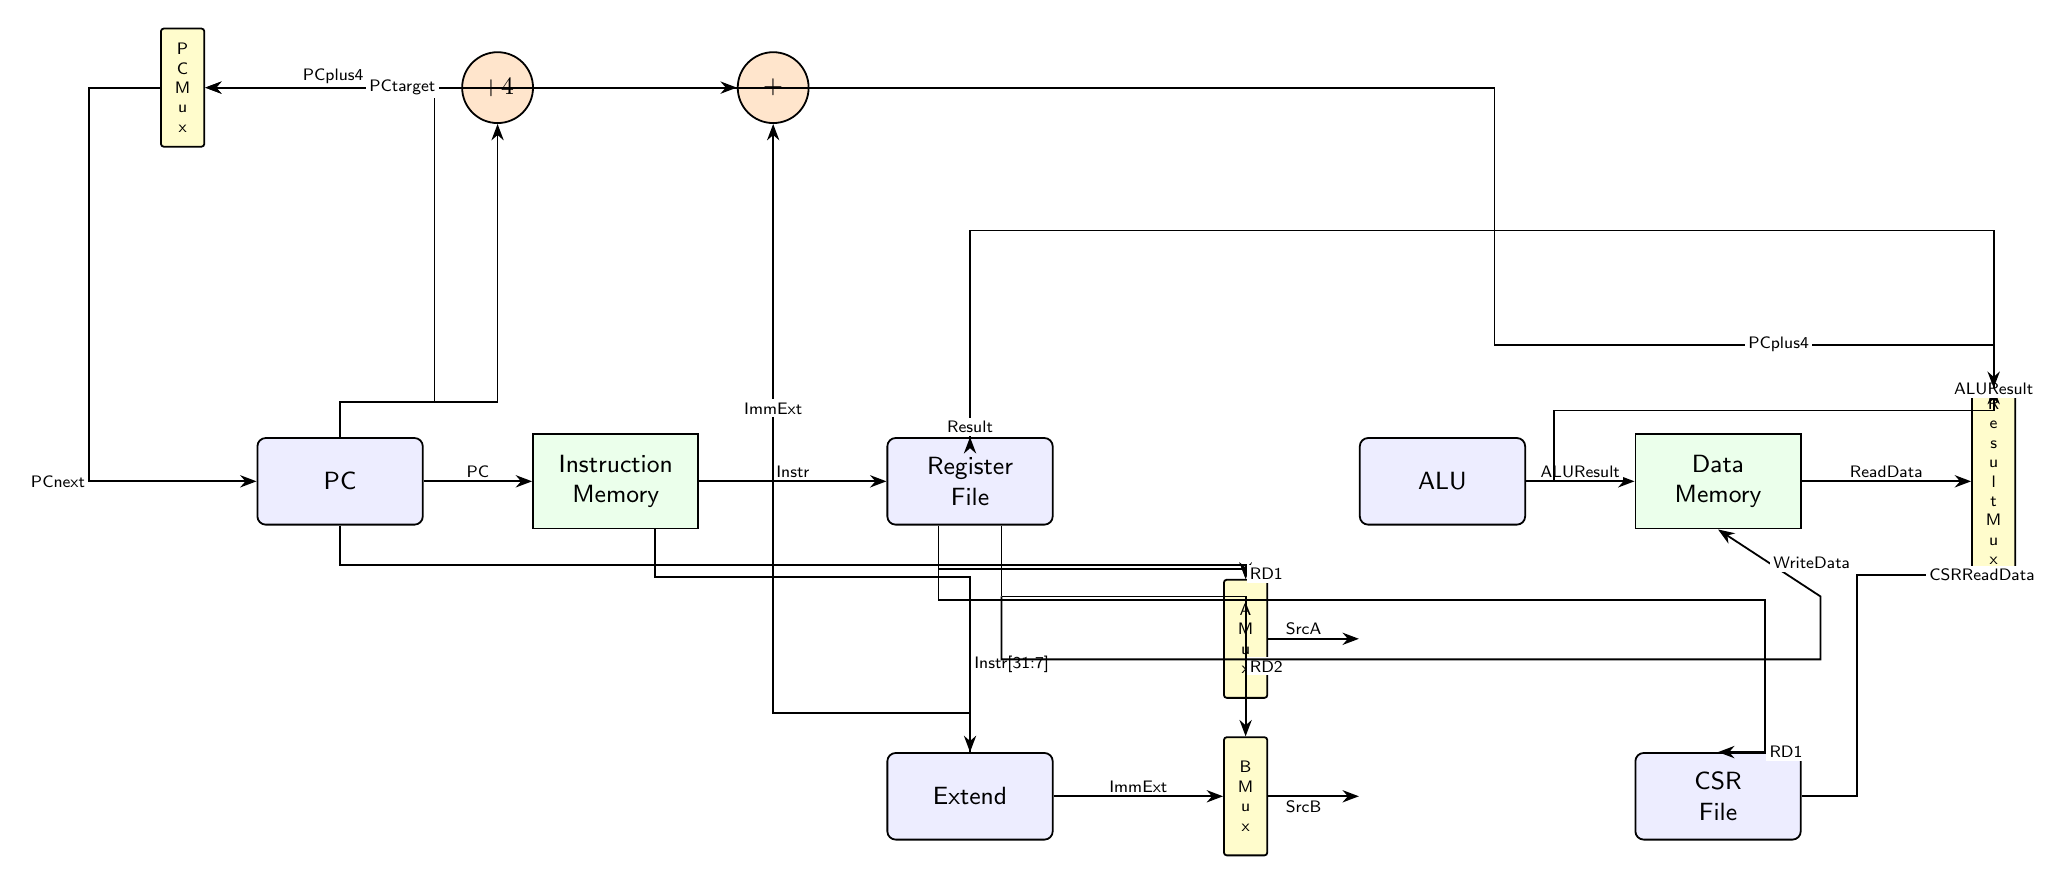
\begin{tikzpicture}[
  >=Stealth, line width=0.65pt,
  %── node styles ─────────────────────────────────────────────────────────────
  fu/.style  = {draw, fill=blue!7,   rectangle, rounded corners=3pt,
                minimum width=2.1cm, minimum height=1.1cm,
                align=center, font=\small\sffamily},
  mem/.style = {draw, fill=green!8,  rectangle,
                minimum width=2.1cm, minimum height=1.2cm,
                align=center, font=\small\sffamily},
  mux/.style = {draw, fill=yellow!20, rectangle, rounded corners=1pt,
                minimum width=0.55cm, minimum height=1.5cm,
                align=center, font=\fontsize{6}{7}\selectfont\sffamily},
  add/.style = {draw, fill=orange!20, circle,
                minimum size=0.9cm, inner sep=0pt,
                font=\small\sffamily},
  %── wire label ──────────────────────────────────────────────────────────────
  wl/.style  = {font=\fontsize{6.5}{8}\selectfont\sffamily,
                fill=white, inner sep=1.2pt, midway},
]

%─────────────────────────────────────────────────────────────────────────────
% NODE PLACEMENT
%   x: 0   3   7  11  15  18.5  22
%   y: 0 (main), +5 (PC adders), -4 (Extend / ALU-src muxes / CSR)
%─────────────────────────────────────────────────────────────────────────────

% ── row y = 0  (main data path) ──────────────────────────────────────────────
\node[fu]  (PC)   at ( 0,    0) {PC};
\node[mem] (IMEM) at ( 3.5,  0) {Instruction\\Memory};
\node[fu]  (RF)   at ( 8,    0) {Register\\File};
\node[fu]  (ALU)  at (14,    0) {ALU};
\node[mem] (DMEM) at (17.5,  0) {Data\\Memory};
\node[mux] (RMUX) at (21,    0) {R\\e\\s\\u\\l\\t\\M\\u\\x};

% ── row y = +5  (PC adders and PC mux) ───────────────────────────────────────
\node[add] (PP4)   at ( 2,    5) {\small$+4$};
\node[add] (PTGT)  at ( 5.5,  5) {\small$+$};
\node[mux] (PCMUX) at (-2,    5) {P\\C\\M\\u\\x};

% ── row y = −4  (Extend, SrcA mux, SrcB mux, CSR file) ──────────────────────
\node[fu]  (EXT)  at ( 8,   -4) {Extend};
\node[mux] (AMUX) at (11.5, -2) {A\\M\\u\\x};
\node[mux] (BMUX) at (11.5, -4) {B\\M\\u\\x};
\node[fu]  (CSR)  at (17.5, -4) {CSR\\File};

%─────────────────────────────────────────────────────────────────────────────
% WIRES
%─────────────────────────────────────────────────────────────────────────────

%── 1.  PC → Instruction Memory ───────────────────────────────────────────────
\draw[->] (PC.east) -- node[wl,above]{PC} (IMEM.west);

%── 2.  Instruction Memory → Register File  (Instr bus) ───────────────────────
\draw[->] (IMEM.east) -- node[wl,above]{Instr} (RF.west);

%── 3.  Instruction Memory → Extend  (bits 31:7) ──────────────────────────────
\coordinate (imem_s) at ($(IMEM.south)+(0.5,0)$);
\draw[->] (imem_s) -- ++(0,-0.6) -| node[wl,right,near end]{Instr[31:7]} (EXT.north);

%── 4.  PC → PC+4 adder ───────────────────────────────────────────────────────
\coordinate (pc_n) at ($(PC.north)+(0,0)$);
\draw[->] (pc_n) -- ++(0,0.45) -| (PP4.south);

%── 5.  PC → PC_Target adder  (same upward tap) ──────────────────────────────
\draw[->] (pc_n) -- ++(0,0.45) -- ++(1.2,0) |- (PTGT.west);

%── 6.  PC → SrcA mux  (AUIPC: PCSrcA selects PC as ALU operand A) ────────────
\draw[->] (PC.south) -- ++(0,-0.5) -| node[wl,right,near end]{PC} (AMUX.north);

%── 7.  Extend → PC_Target adder ─────────────────────────────────────────────
\draw[->] (EXT.north) -- ++(0,0.5) -| node[wl,above,near end]{ImmExt} (PTGT.south);

%── 8.  Extend → SrcB (ALU_Mux) ─────────────────────────────────────────────
\draw[->] (EXT.east) -- node[wl,above]{ImmExt} (BMUX.west |- EXT);

%── 9.  PP4 → PC_Mux  (upper port) ───────────────────────────────────────────
\draw[->] (PP4.west)  -- node[wl,above]{PCplus4} (PCMUX.east |- PP4);

%── 10. PC_Target → PC_Mux  (lower port) ─────────────────────────────────────
\draw[->] (PTGT.west) -- ++(-0.8,0) |- node[wl,left,near end]{PCtarget}
          (PCMUX.east |- PTGT);

%── 11. PC_Mux → PC  (PCnext loop-back) ──────────────────────────────────────
\draw[->] (PCMUX.west) -- ++(-0.9,0) |- node[wl,left]{PCnext} (PC.west);

%── 12. Register File RD1 → SrcA mux ─────────────────────────────────────────
\coordinate (rd1_tap) at ($(RF.south)+(-0.4,0)$);
\draw[->] (rd1_tap) -- ++(0,-0.55) -| node[wl,right,near end]{RD1} (AMUX.north);

%── 13. Register File RD2 → SrcB (ALU_Mux) ───────────────────────────────────
\coordinate (rd2_tap) at ($(RF.south)+(0.4,0)$);
\coordinate (rd2_fork) at ($(rd2_tap)+(0,-0.9)$);
\draw (rd2_tap) -- (rd2_fork);
\draw[->] (rd2_fork) -| node[wl,right,near end]{RD2} (BMUX.north);

%── 14. Register File RD2 → Data Memory  (WriteData for stores) ───────────────
%       Route below the lower nodes so it does not cross anything.
\draw[->] (rd2_fork) -- ++(0,-0.8) -- ++(10.4,0) -- ++(0,0.8)
          -- node[wl,right]{WriteData} (DMEM.south);

%── 15. SrcA mux → ALU port A ────────────────────────────────────────────────
\draw[->] (AMUX.east) -- ++(0.45,0) |- node[wl,above]{SrcA}
          (ALU.west |- AMUX.east);

%── 16. SrcB mux → ALU port B ────────────────────────────────────────────────
\draw[->] (BMUX.east) -- ++(0.45,0) |- node[wl,below]{SrcB}
          (ALU.west |- BMUX.east);

%── 17. ALU → Data Memory  (address) ─────────────────────────────────────────
\draw[->] (ALU.east) -- node[wl,above]{ALUResult} (DMEM.west);

%── 18. ALU result tap → Result Mux  (bypass read data) ──────────────────────
\coordinate (alu_tap) at ($(ALU.east)+(0.35,0)$);
\draw[->] (alu_tap) -- ++(0,0.9) -|
          node[wl,above,near end]{ALUResult} (RMUX.north);

%── 19. Data Memory → Result Mux ─────────────────────────────────────────────
\draw[->] (DMEM.east) -- node[wl,above]{ReadData} (RMUX.west |- DMEM);

%── 20. PP4 → Result Mux  (JAL/JALR return address) ──────────────────────────
\draw[->] (PP4.east) -- ++(12.2,0) |- node[wl,right,near end]{PCplus4}
          ($(RMUX.north)+(0,0.55)$) -- (RMUX.north);

%── 21. CSR File read data → Result Mux ──────────────────────────────────────
\draw[->] (CSR.east) -- ++(0.7,0) |-
          node[wl,right,near end]{CSRReadData} (RMUX.south);

%── 22. Register File RD1 → CSR write data ───────────────────────────────────
\draw[->] (rd1_tap) -- ++(0,-0.55) -- ++(0,-0.4) -- ++(10.5,0) |-
          node[wl,right]{RD1} (CSR.north);

%── 23. Result Mux → Register File  (writeback over the top) ─────────────────
\draw[->] (RMUX.north) -- ++(0,2.0) -- ++(-13,0) |-
          node[wl,above]{Result} (RF.north);

\end{tikzpicture}
\end{document}
